\section{Performance of the Spherical Harmonics Analysis in Separating 0\nbb-decay from \B~Background.}
\label{sec:performance}

%% Taritree (9/20/16): is it multipole or multiple?

The separation of signal and background comes almost entirely from the
first two multiple moments, $l=0$ and $l=1$. However, higher multiple
moments are needed for the event-by-event normalization of the power spectrum
$S_l$ (Eq.~\ref{eq6}). In the following, we choose to calculate the
power spectrum $s_l$ up to l=3 and use only the normalized variables $S_0$
and $S_1$, where the normalization is given by

\begin{eqnarray}
\label{eq7}
S_{0,1} = \frac{s_{0,1}}{\sum_{l=0}^{3} s_l}.
\end{eqnarray}

As discussed below, a linear combination of $S_0$ and $S_1$ can be
used to construct a single discriminant, $S_{01}$. 
Distributions of $S_{01}$ for 0\nbb~and \B~events can be used to optimize
detector design parameters, as described below.

\subsection{Central events with no uncertainty on the vertex position}

To illustrate the technique, we initially evaluate 
the performance of the spherical harmonics
analysis in the idealized case of events at the center of the
detector with perfect reconstruction of the event vertex
position. For such events, a time cut of 33.5~ns on the PE arrival
time can be applied to obtain an `early PE' sample that contains a
high fraction of Cherenkov PEs. The default QE of xx for Cherenkov
light and xx for scintillation light and xx\% photo-coverage are used
in the simulation.

A comparison of $S_0$ and $S_1$ distributions for 0\nbb-decay signal
and \B~background events is shown in Fig.~\ref{fig:S_vs_energy}.  Both
variables provide a noticeable separation between signal and
background. We note that in the energy range of interest, the
$S_l$'s do not strongly depend on the energy deposited in the
detector, i.e. information contained in the normalized power
spectrum is complimentary to the energy measurements. 

\begin{figure*}[h]
\centering
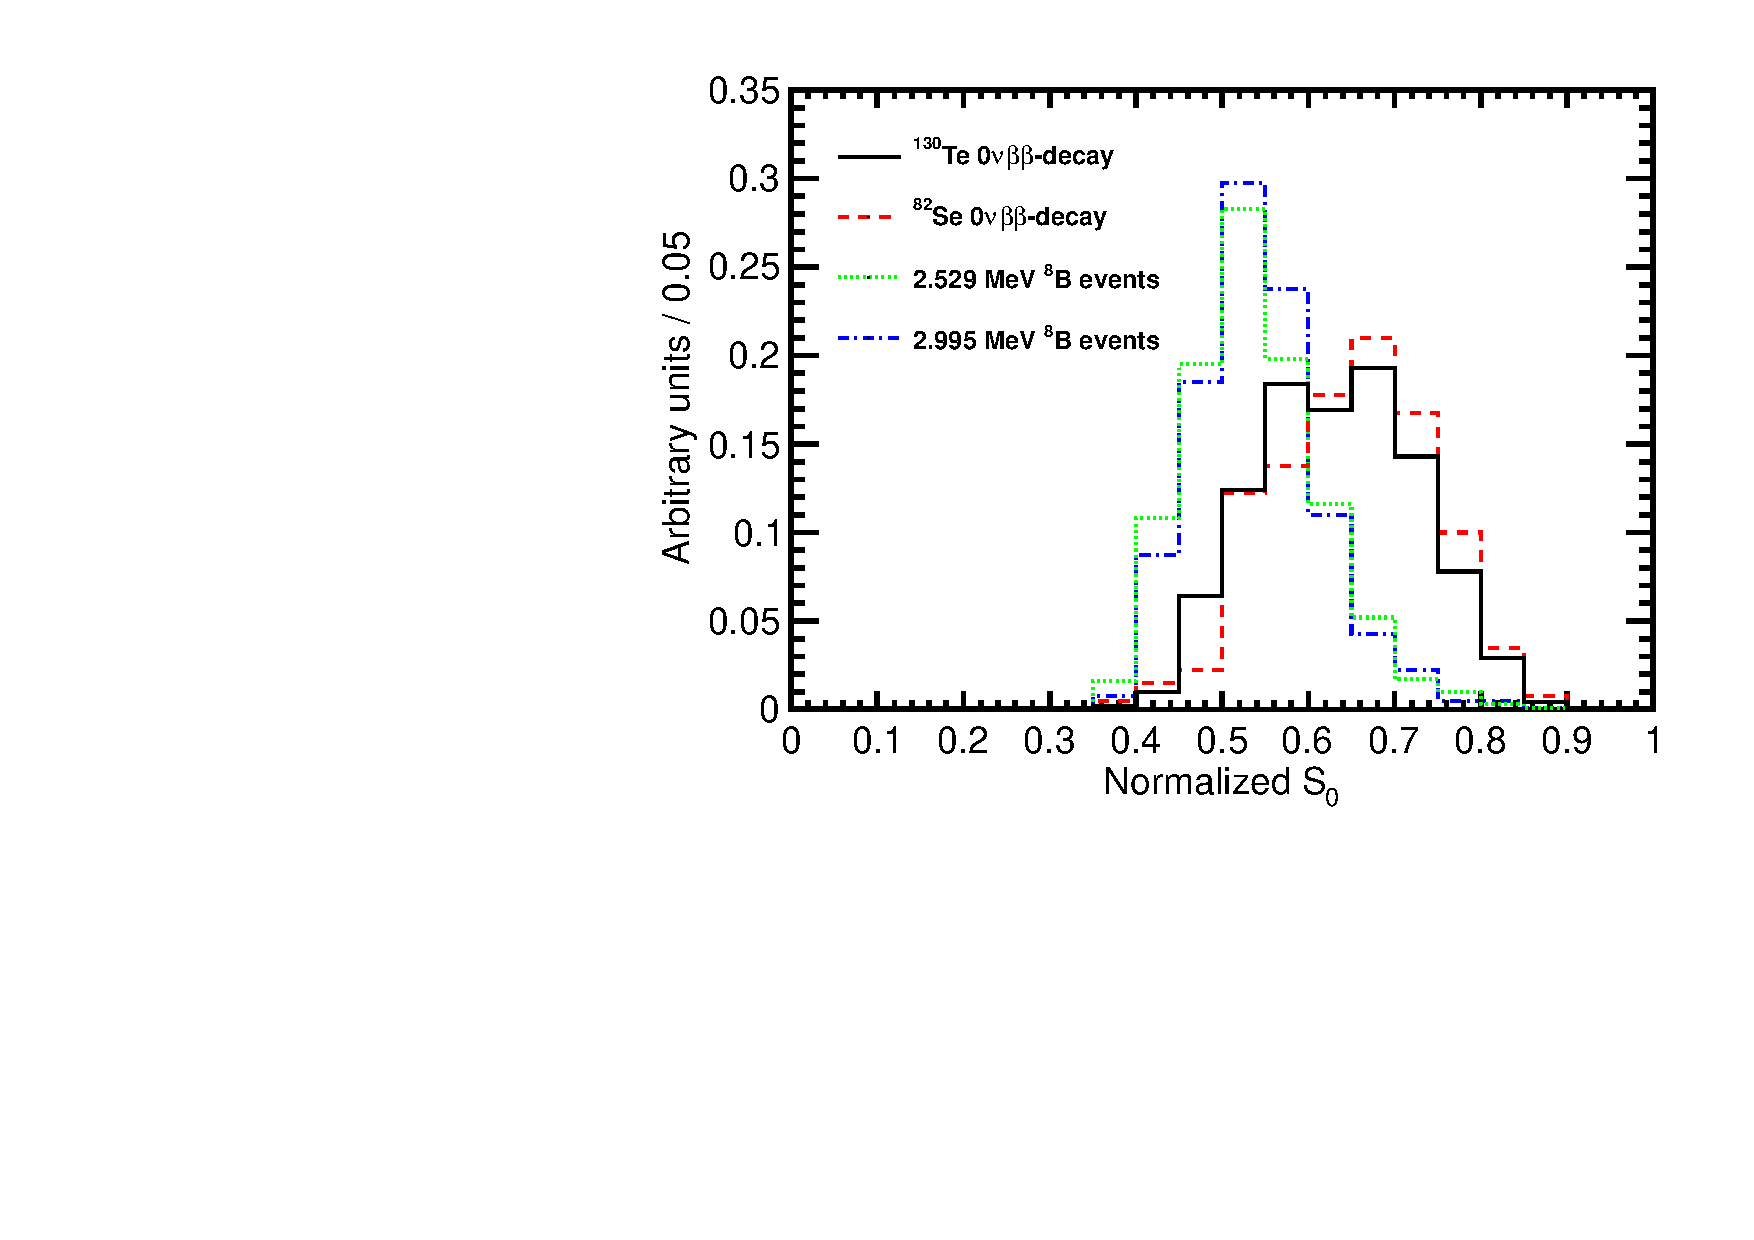
\includegraphics[width=0.49\textwidth]{hS0.pdf}
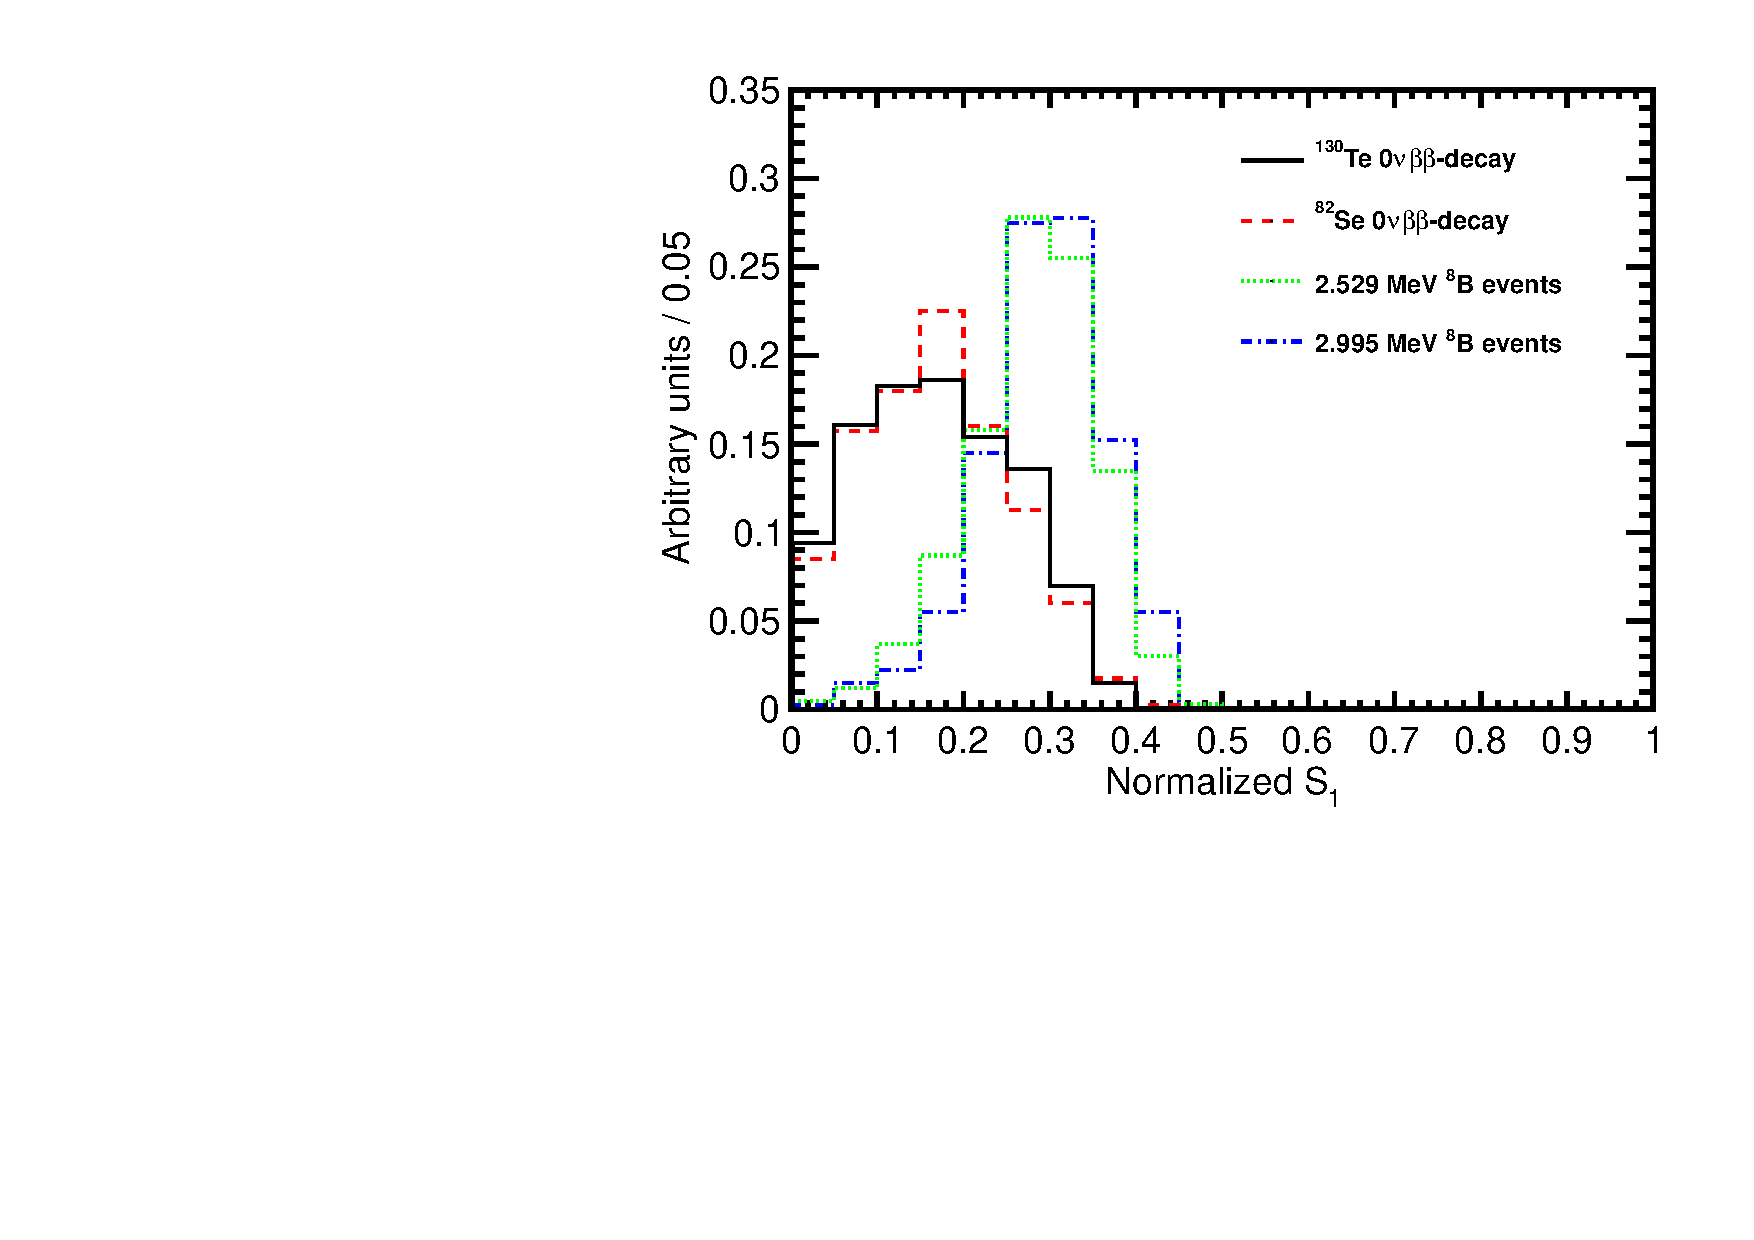
\includegraphics[width=0.49\textwidth]{hS1.pdf}
\caption{Results from the idealized case of central events at the
  detector origin( i.e. perfect vertex reconstruction); a time cut of 33.5~ns
  on the PE arrival time is applied. The default QE and xx\%
  photo-coverage are used in the simulation.  (\emph{Left}) $S_0$ and
  $S_1$ (\emph{right}) distributions for 1000 simulated 0\nbb-decay
  signal and \B~background events.  Two different isotopes are
  compared, $^{130}$Te and $^{82}$Se. The corresponding kinetic
  energies of background \B~neutrino single electrons are 2.53 MeV and
  3.00 MeV.}
\label{fig:S_vs_energy}
\end{figure*}

The left-hand panel in Fig.~\ref{fig:SL_Te_33p5ns_center} compares
scatter plots of the first two components of the power spectrum, $S_0$
and $S_1$, for signal and background. In order to illustrate the
separation between $^{130}$Te and $^{8}$B events, a linear combination
of variables $S_0$ and $S_1$ is constructed as follows~\footnote{A
multi-variate event-by-event analysis will have more discriminatory
power than this simple 1-dimensional separation, but in the absence of
a real detector is a waste of time~\cite{goldberger_watson}.}.
%% Taritree (9/20/16): Reconsider using "a waste of time" for something less colloquial.

First, a linear fit to $S_0$ = $A \cdot S_1 + B$, of all points on the
scatter plot is performed, as shown by the dashed line in the left-hand
panel in Fig.~\ref{fig:SL_Te_33p5ns_center}. A 1-dimensional (1-D) variable
$S_{01}$ is defined as $S_{01} = S_1 \cdot cos(\theta) + S_0 \cdot
sin(\theta)$, where $tan(\theta)$=$A$. The right-hand panel in
Fig.~\ref{fig:SL_Te_33p5ns_center} compares distributions of $S_{01}$
for 0\nbb-decay signal and \B~background. These 1-D histograms for
$S_{01}$ represent the projection of the points on the scatter plot
onto the fitted line.

To quantify the separation between the signal and background we
calculate the area of the overlap in the $S_{01}$ distributions,
$I_{overlap}$. There is no separation if $I_{overlap}$=1, and there is
a 100\% separation if
$I_{overlap}$=0. Figure~\ref{fig:SL_Te_33p5ns_center} shows the
separation of this simple algorithm based on the shape of the early PE
sample; the overlap between signal and background is
$I_{overlap}$=0.52. At an efficiency for the signal of
70\% we find a rejection factor of 4.6.

%The separation $\frac{\epsilon}{I} = \frac{0.915}{0.521} = 1.76$.


\begin{figure*}[h]
  \centering
  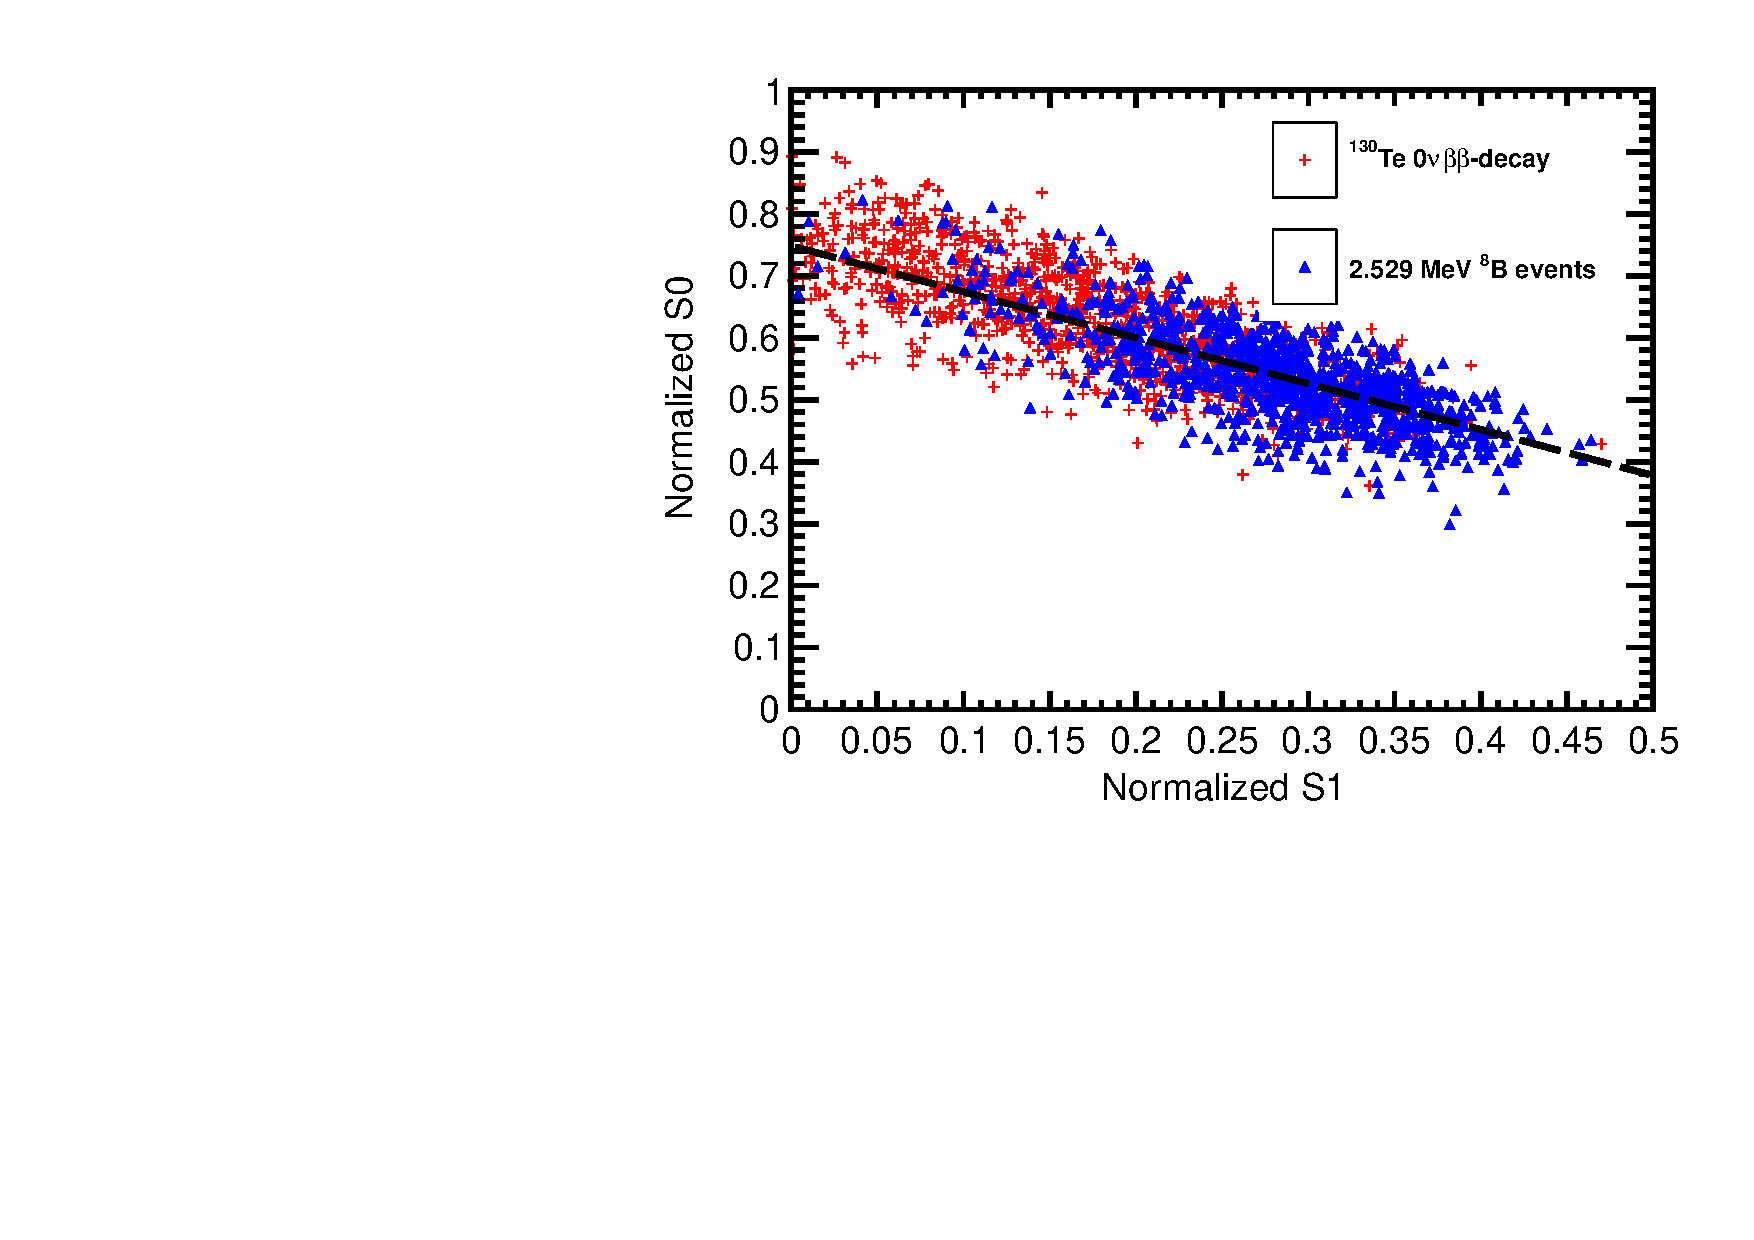
\includegraphics[width=0.49\textwidth]{hS0vsS1_Te130_1el_allLight_VtxSmear0cm_VtxShiftX0cm_33p5ns_center.pdf}
  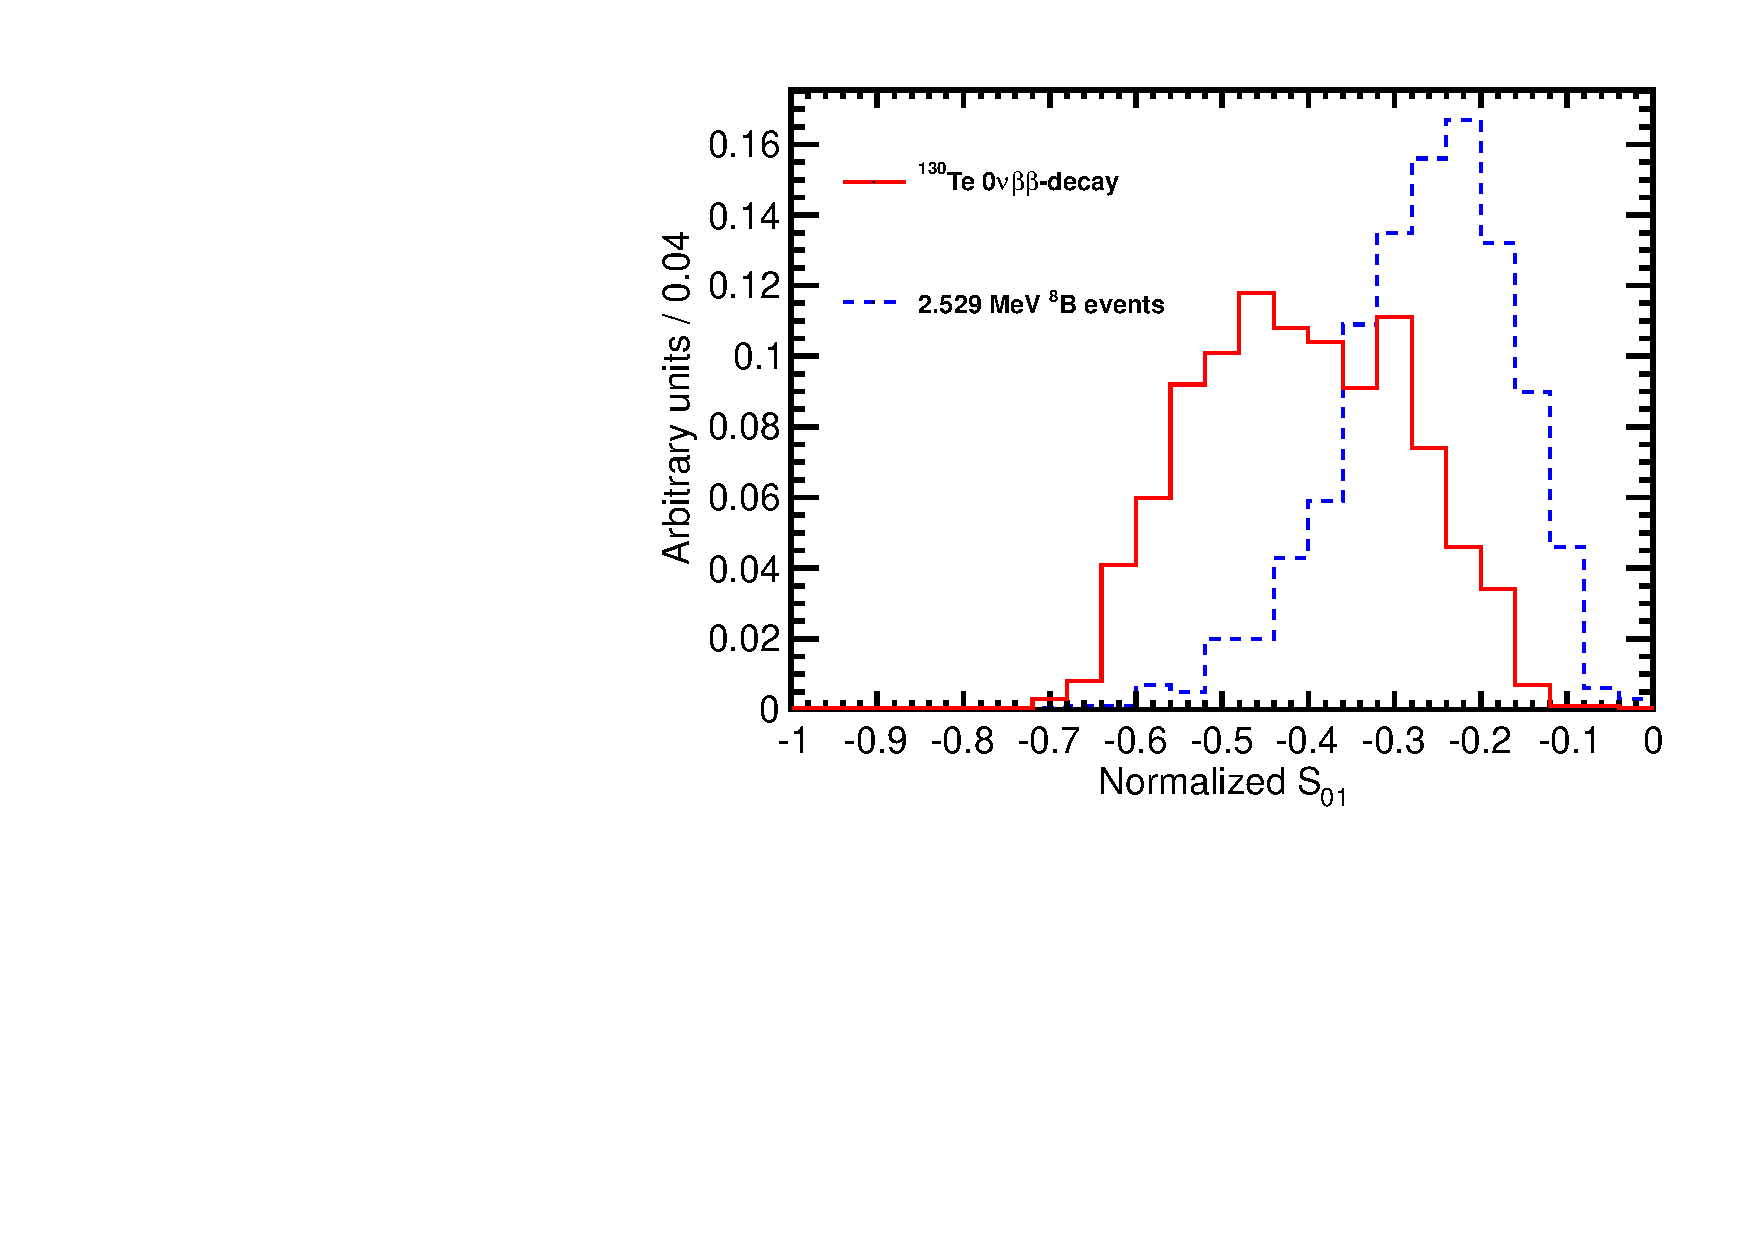
\includegraphics[width=0.49\textwidth]{hS01_allLight_VtxSmear0cm_VtxShiftX0cm_33p5ns_center.pdf}
  \caption{\emph{Left:} Scatter plot of the moments $S_0$ versus $S_1$
    for a simulation of 1000 signal (\emph{red crosses}) and
    background (\emph{blue triangles}), for the idealized case of
    central events assuming perfect reconstruction of the vertex
    position. A time cut of 33.5~ns on the PE arrival time is
    applied. The default QE and xx\% photo-coverage is used in the
    simulation.  The black dashed line corresponds to a linear fit for
    $S_{01}$.  \emph{Right:} Comparison of the $S_{01}$ distribution
    between signal (\emph{red solid line}) and background (\emph{blue
    dashed line}).  $I_{overlap}$=0.52.}
\label{fig:SL_Te_33p5ns_center}
\end{figure*}

%separation = 0.915454
%overlap = 0.521

\subsection{Experimental challenges: chromatic dispersion and 
vertex resolution}

Samples of 1000 events each of signal and background were simulated
with origins distributed throughout the whole fiducial volume of the
detector with a vertex resolution of 3cm found from our earlier study of
reconstruction\cite{Aberle2014}.  For the general case, even
significantly delayed scintillation photons can reach the side of the
detector that is closer to the vertex much earlier than Cherenkov
photons traveling to the opposite side of the detector. The time cut
thus has to take into account the total distance traveled by each
individual photon.

In general, the $S_1$ component of the spherical harmonics power
spectrum is higher for asymmetric distributions and lower for
symmetric distributions (e.g., compare the back-to-back and single
electron topologies in
Fig.~\ref{fig:ThreeTopologies_Display_5MeV}). If a vertex is shifted
in the direction opposite to the track of the electron, the
differential time cut selects more scintillation photons that are
emitted in the direction of the electron track.  Scintillation photons
would enhance the forward asymmetry of the early PE sample, which
in turn would move $S_1$ to higher values.  Moreover, $S_1=$~0 for a
distribution with perfect symmetry with respect to the center of the
sphere.  If a vertex is shifted in the same direction as the direction
of the electron, the differential time cut selects more scintillation
photons that are emitted in the direction opposite to the electron
track. The asymmetry of Cherenkov PEs would then be counter-balanced
by scintillation PEs, which in turn, would move $S_1$ to lower values.


\subsection{Events in a fiducial volume with an uncertainty on the vertex position}
We find that in the default detector model the separation power of
the spherical harmonics analysis is significantly reduced when chromatic
dispersion and vertex resolution are taken into account.

We simulated 1000 signal and background events that have their
vertices uniformly distributed within a fiducial volume of $R<3$~m,
where $R$ is the distance between the event vertex and the center of
the detector. To implement an uncertainty on the vertex reconstruction
we apply a 3~cm smearing around the actual vertex position for each
simulated event. The smearing is done along $x$, $y$, and $z$
directions with three independent Gaussian distributions of the same
width, $\sigma_x = \sigma_y = \sigma_z =$3~cm.

Figure~\ref{fig:SL_Te_SmearX3cm_momDT1ns_rndVtx_3p0m} shows the
performance of the spherical harmonics analysis under these more
realistic assumptions. The overlap between signal and background is
$I_{overlap}$=0.79, which means that the separation is 52\% worse than
in an idealized scenario shown in Fig.~\ref{fig:SL_Te_33p5ns_center}.
The spherical harmonics analysis brings little separation between
signal and background in our default detector model after the
chromatic dispersion and vertex resolution are taken into
account. However, properties of the liquid scintillator can be
adjusted to improve the performance of the spherical harmonics
analysis. In the following we show that a single change in the
scintillation rise time improves the separation.
%restores most of the separation power that was shown previously in Fig.~\ref{fig:SL_Te_33p5ns_center}.



\begin{figure*}[h]
  \centering
  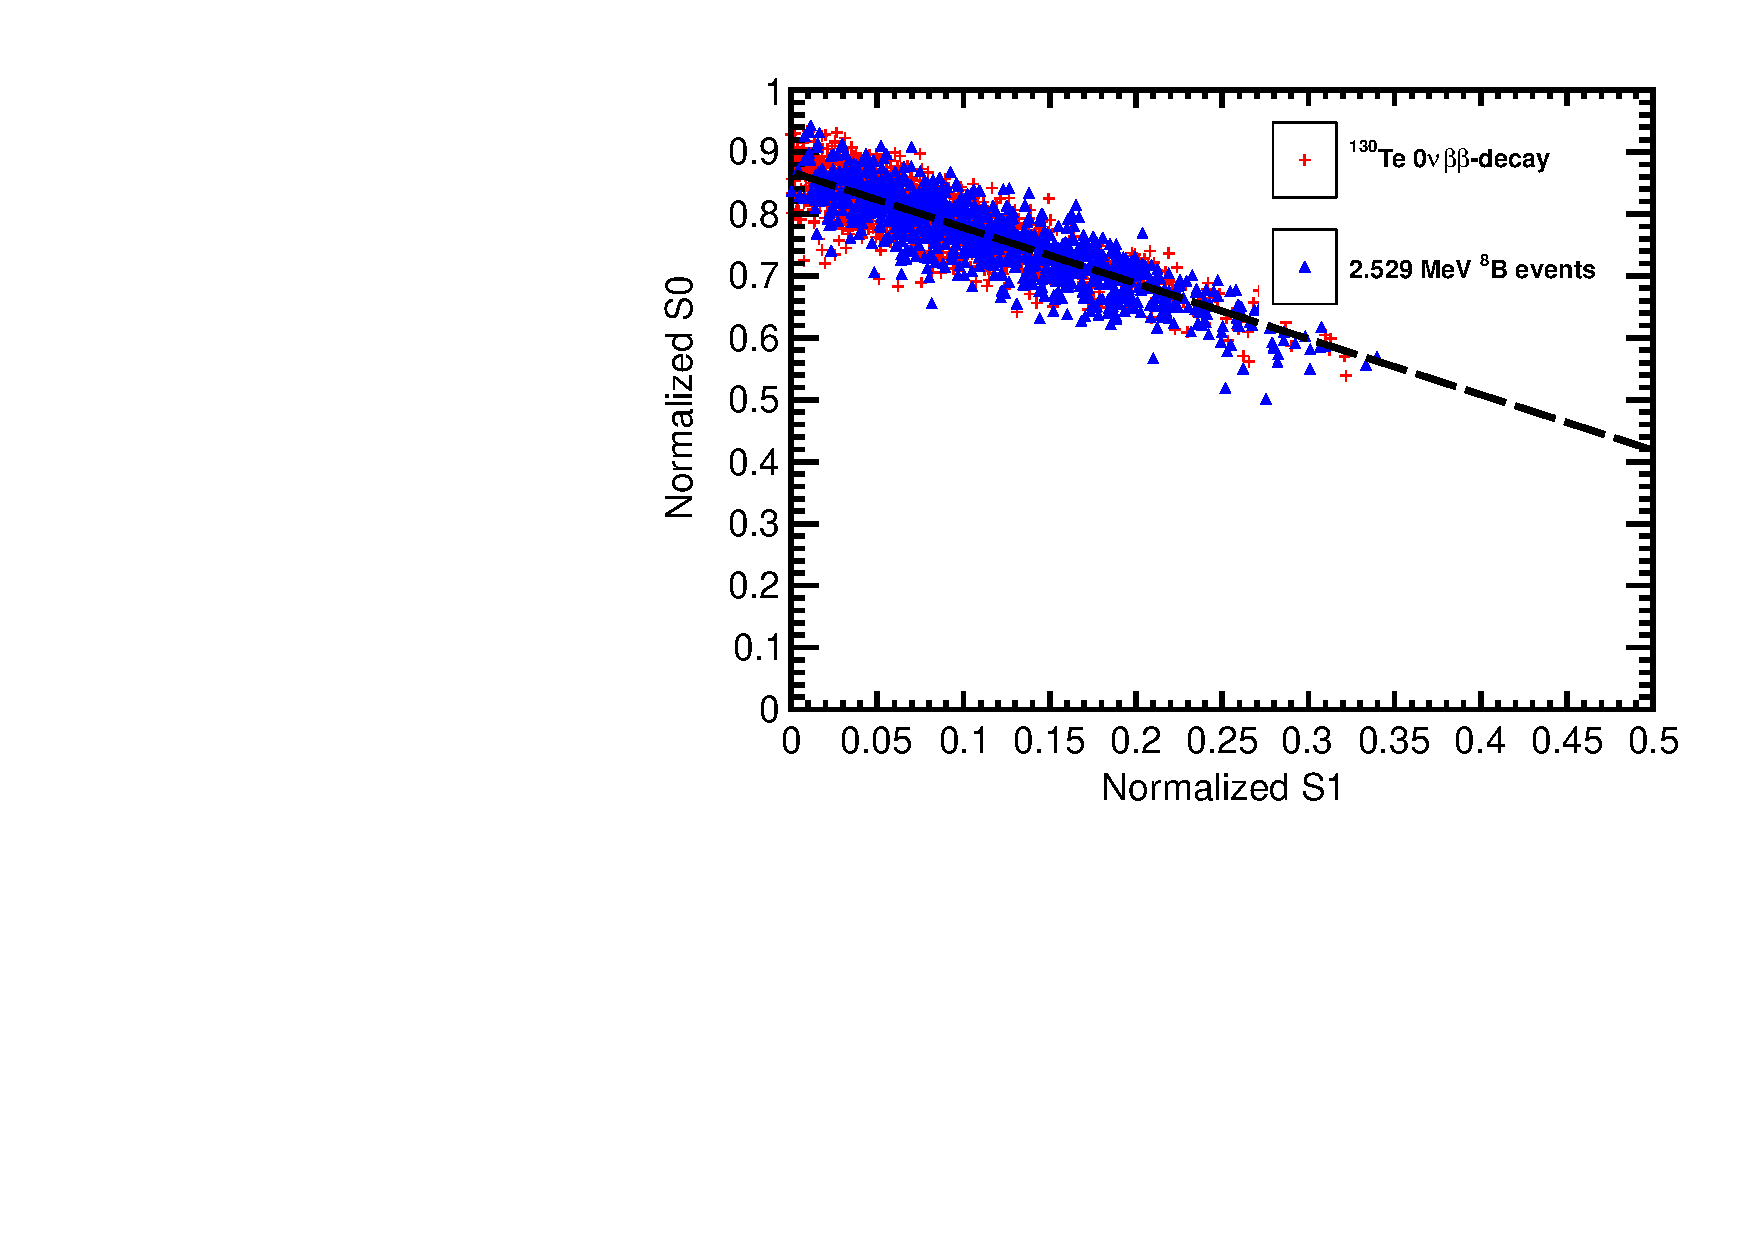
\includegraphics[width=0.49\textwidth]{hS0vsS1_Te130_1el_allLight_VtxSmear3cm_VtxShiftX0cm_momDT1p0ns_rndVtx_3p0mSphere.pdf}
  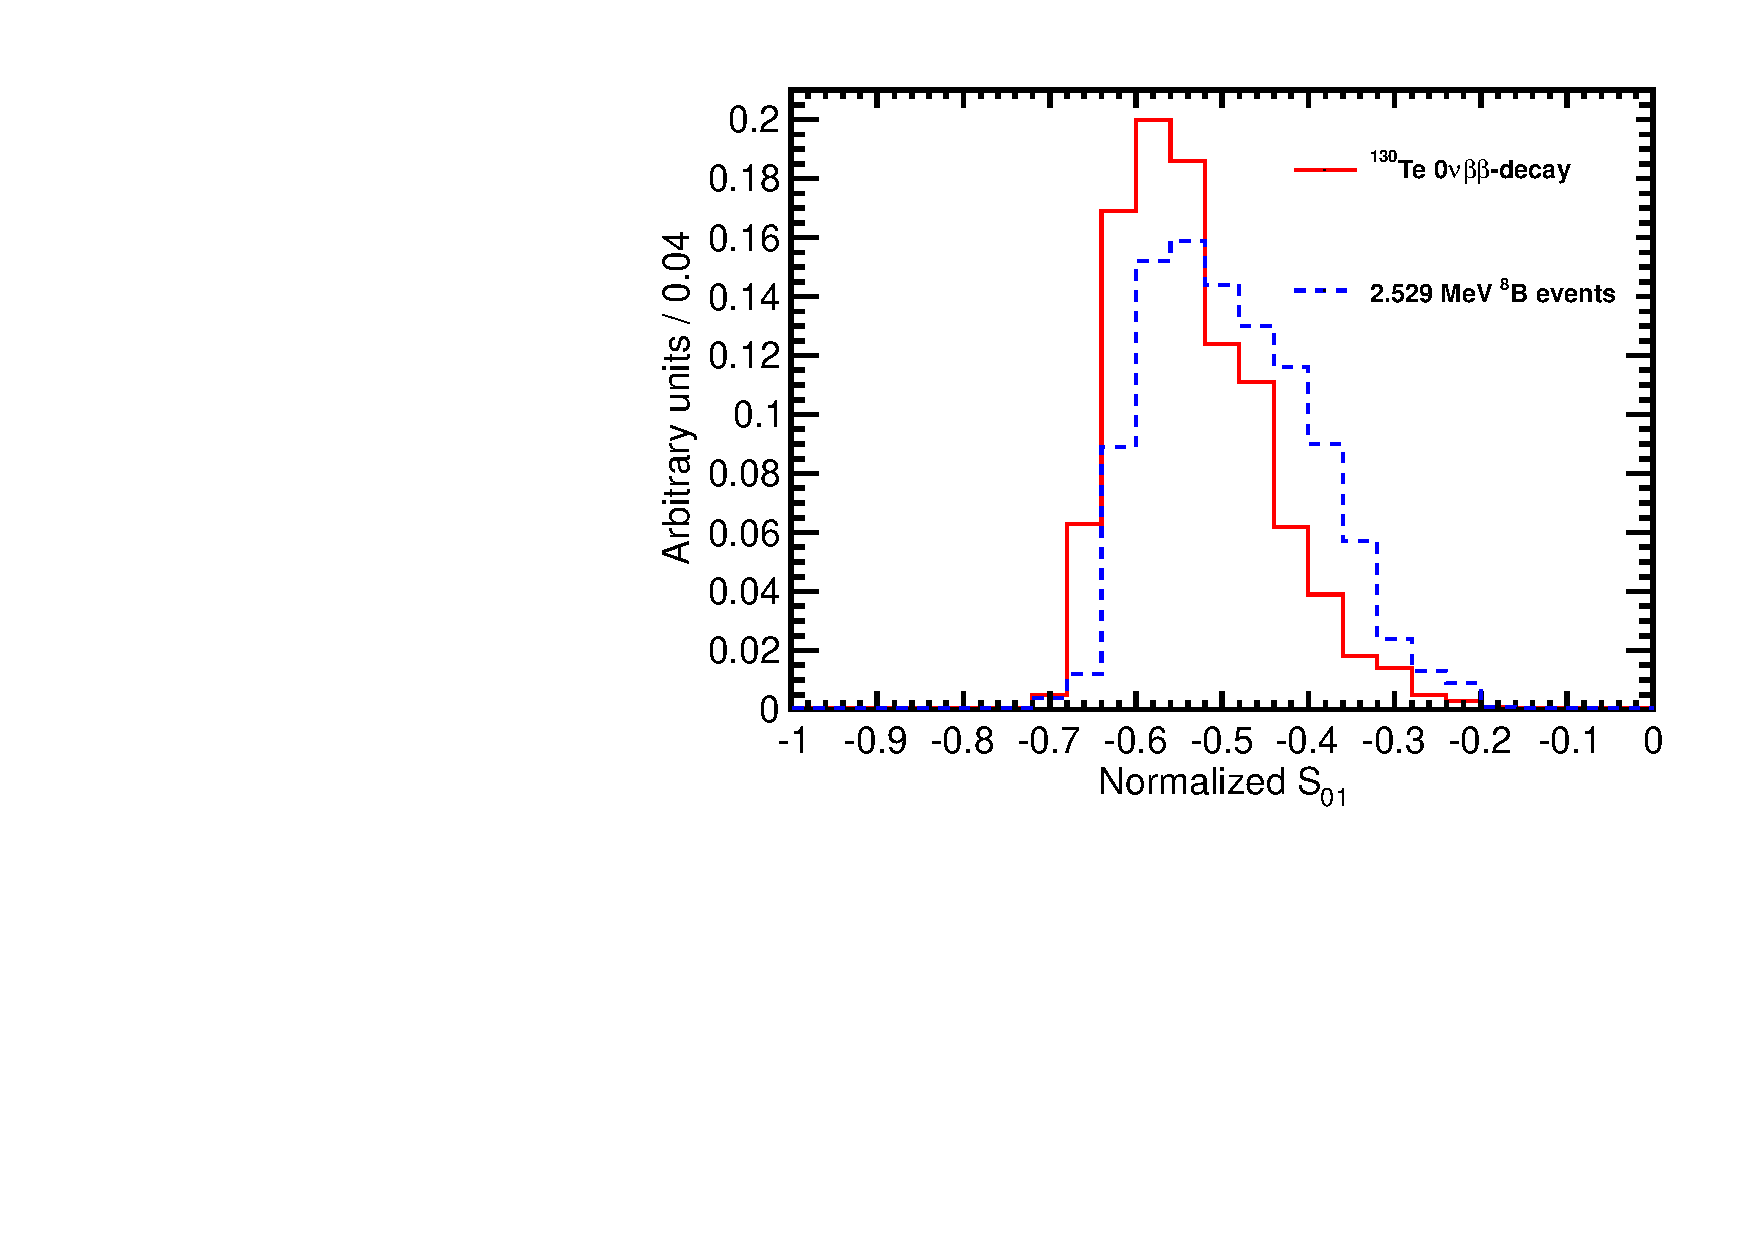
\includegraphics[width=0.49\textwidth]{hS01_allLight_VtxSmear3cm_VtxShiftX0cm_momDT1p0ns_rndVtx_3p0mSphere.pdf}
  \caption{\emph{Left:} Scatter plot of $S_0$ versus $S_1$ for a
    simulation of 1000 signal (\emph{red crosses}) and background
    (\emph{blue triangles}) events. Event vertices are uniformly
    distributed within the fiducial volume, $R<3$~m.  The vertex is
    smeared with 3~cm resolution. A differential cut of $\Delta
    t=t^{phot}_{measured} - t^{phot}_{predicted}<$1~ns is applied to
    select the early PE sample.  The default QE and xx\% photo-coverage
    are used in the simulation.  The black dashed line corresponds to a
    linear fit to define the 1-D variable $S_{01}$.
    \emph{Right:} A comparison of the $S_{01}$ distribution between
    signal (\emph{red solid line}) and background (\emph{blue dashed
    line}).  $I_{overlap}$=0.79.}
\label{fig:SL_Te_SmearX3cm_momDT1ns_rndVtx_3p0m}
\end{figure*}

%separation = 0.357271
%overlap = 0.793


\subsection{Importance of the liquid scintillator properties}
The strong dependence on the vertex resolution can be addressed by
choosing a liquid scintillator mixture with a more delayed emission of
scintillation light with respect to Cherenkov light. With a larger
delay in scintillation light, a higher fraction of Cherenkov light can
be maintained in the early PE sample even if a photon track length is
mis-reconstructed due to imprecise reconstruction of the vertex
position. In addition, if the fraction of scintillation light is small
compared to Cherenkov light, the distortions in the uniformity of the
scintillation PE due to a shifted reconstructed vertex position does
not significantly affect the spherical harmonics power
spectrum. Furthermore, the effects due to chromatic dispersion can be
addressed by using liquid scintillators with a narrower emission
spectrum~\cite{Aberle2014}, or red-enhanced
photocathodes~\cite{Aberle2014}.



While the default detector model assumes a scintillation rise time of
$\tau_r=$1~ns, rise times up to $\tau_r=$7~ns can be achieved (see
Ref.~\cite{Minfang_slow_rise_time}). As a test we increased the
scintillation rise time parameter to $\tau_r=$5~ns in the detector
model, with all other parameters kept the same.  Figure
~\ref{fig:SL_Te_SmearX3cm_momDT1ns_rndVtx_3p0m_SciRT5p0ns} shows the
overlap between signal and background is significantly decreased to
$I_{overlap}$=0.64, i.e. the separation is 23\% worse than in the
idealized scenario shown in Fig.~\ref{fig:SL_Te_33p5ns_center} and
23\% better than in the default detector model shown in
Fig.~\ref{fig:SL_Te_SmearX3cm_momDT1ns_rndVtx_3p0m}.

\begin{figure*}[h]
  \centering
  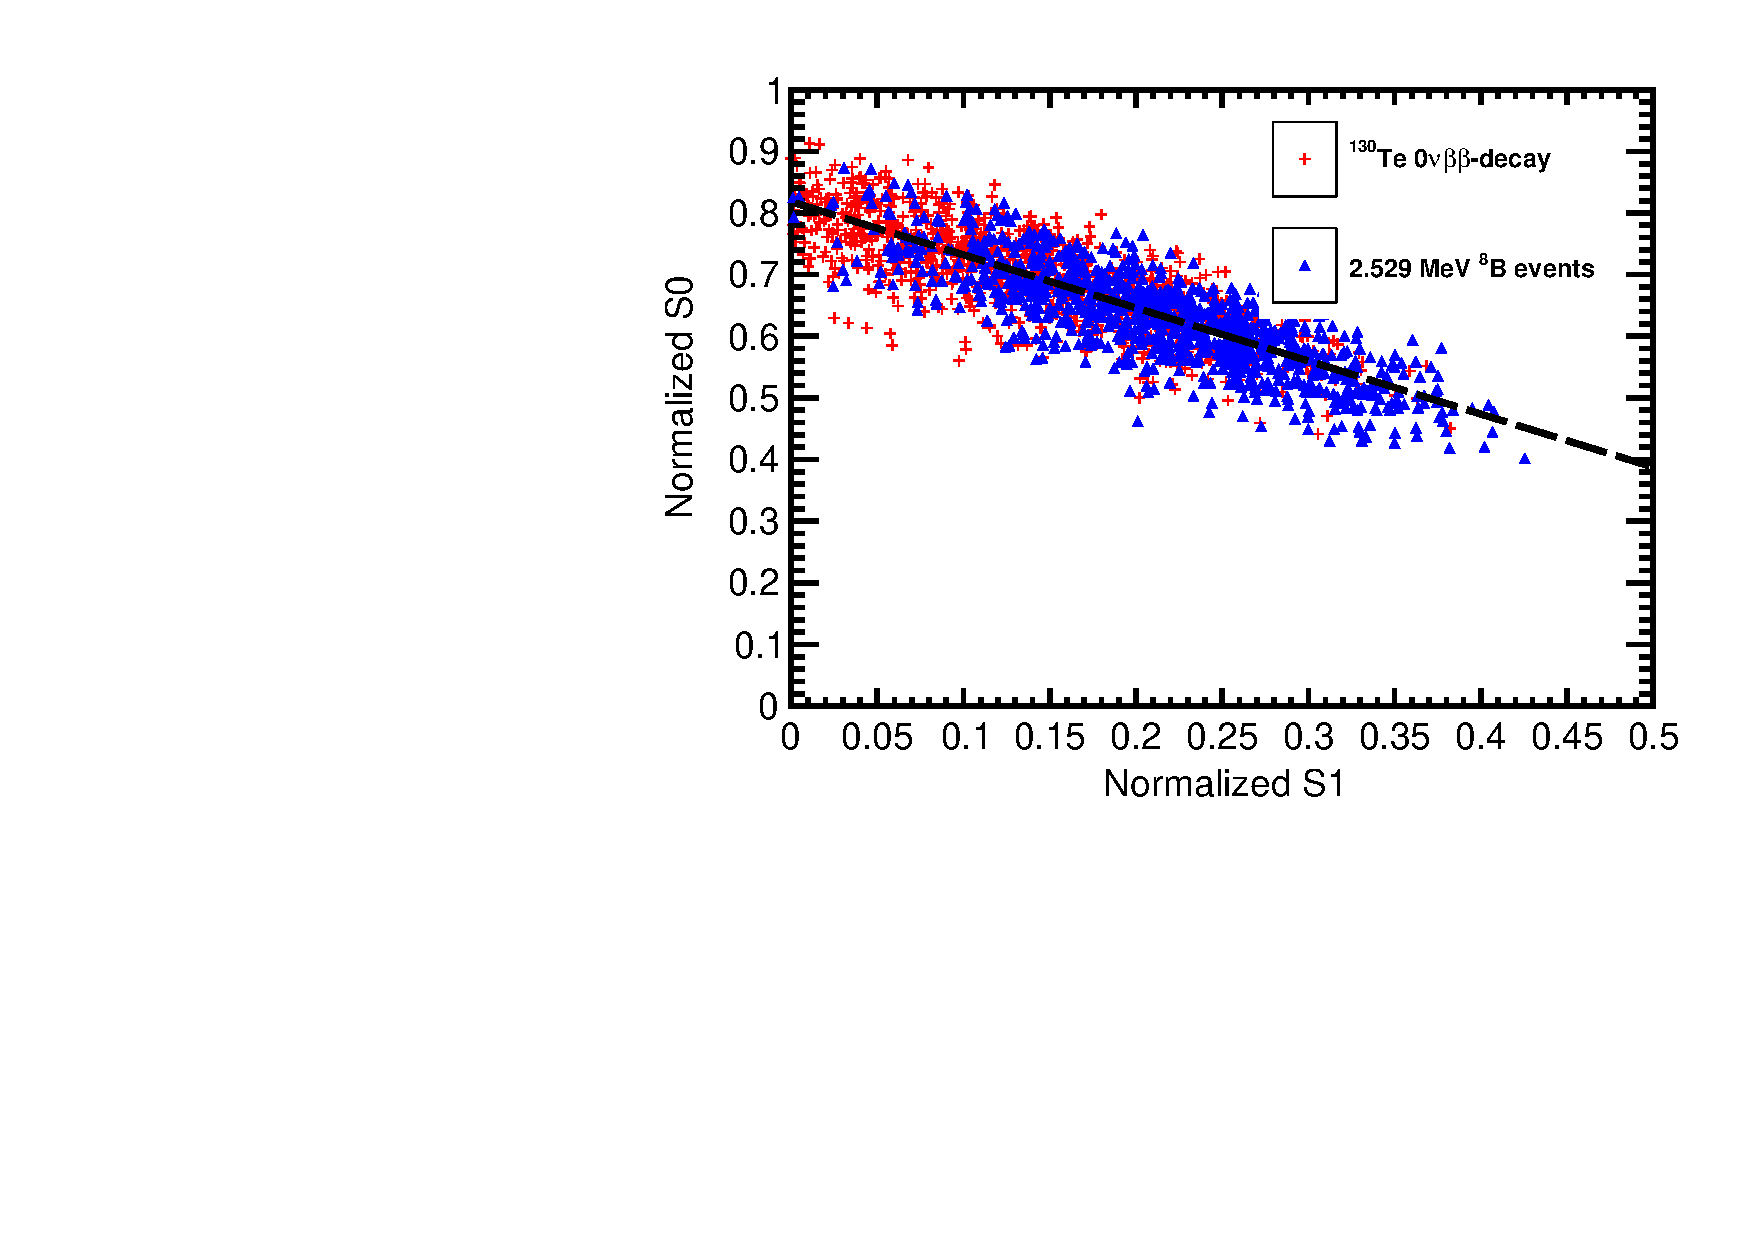
\includegraphics[width=0.49\textwidth]{hS0vsS1_Te130_1el_allLight_VtxSmear3cm_VtxShiftX0cm_momDT1p0ns_rndVtx_3p0mSphere_SciRT5p0ns} 
  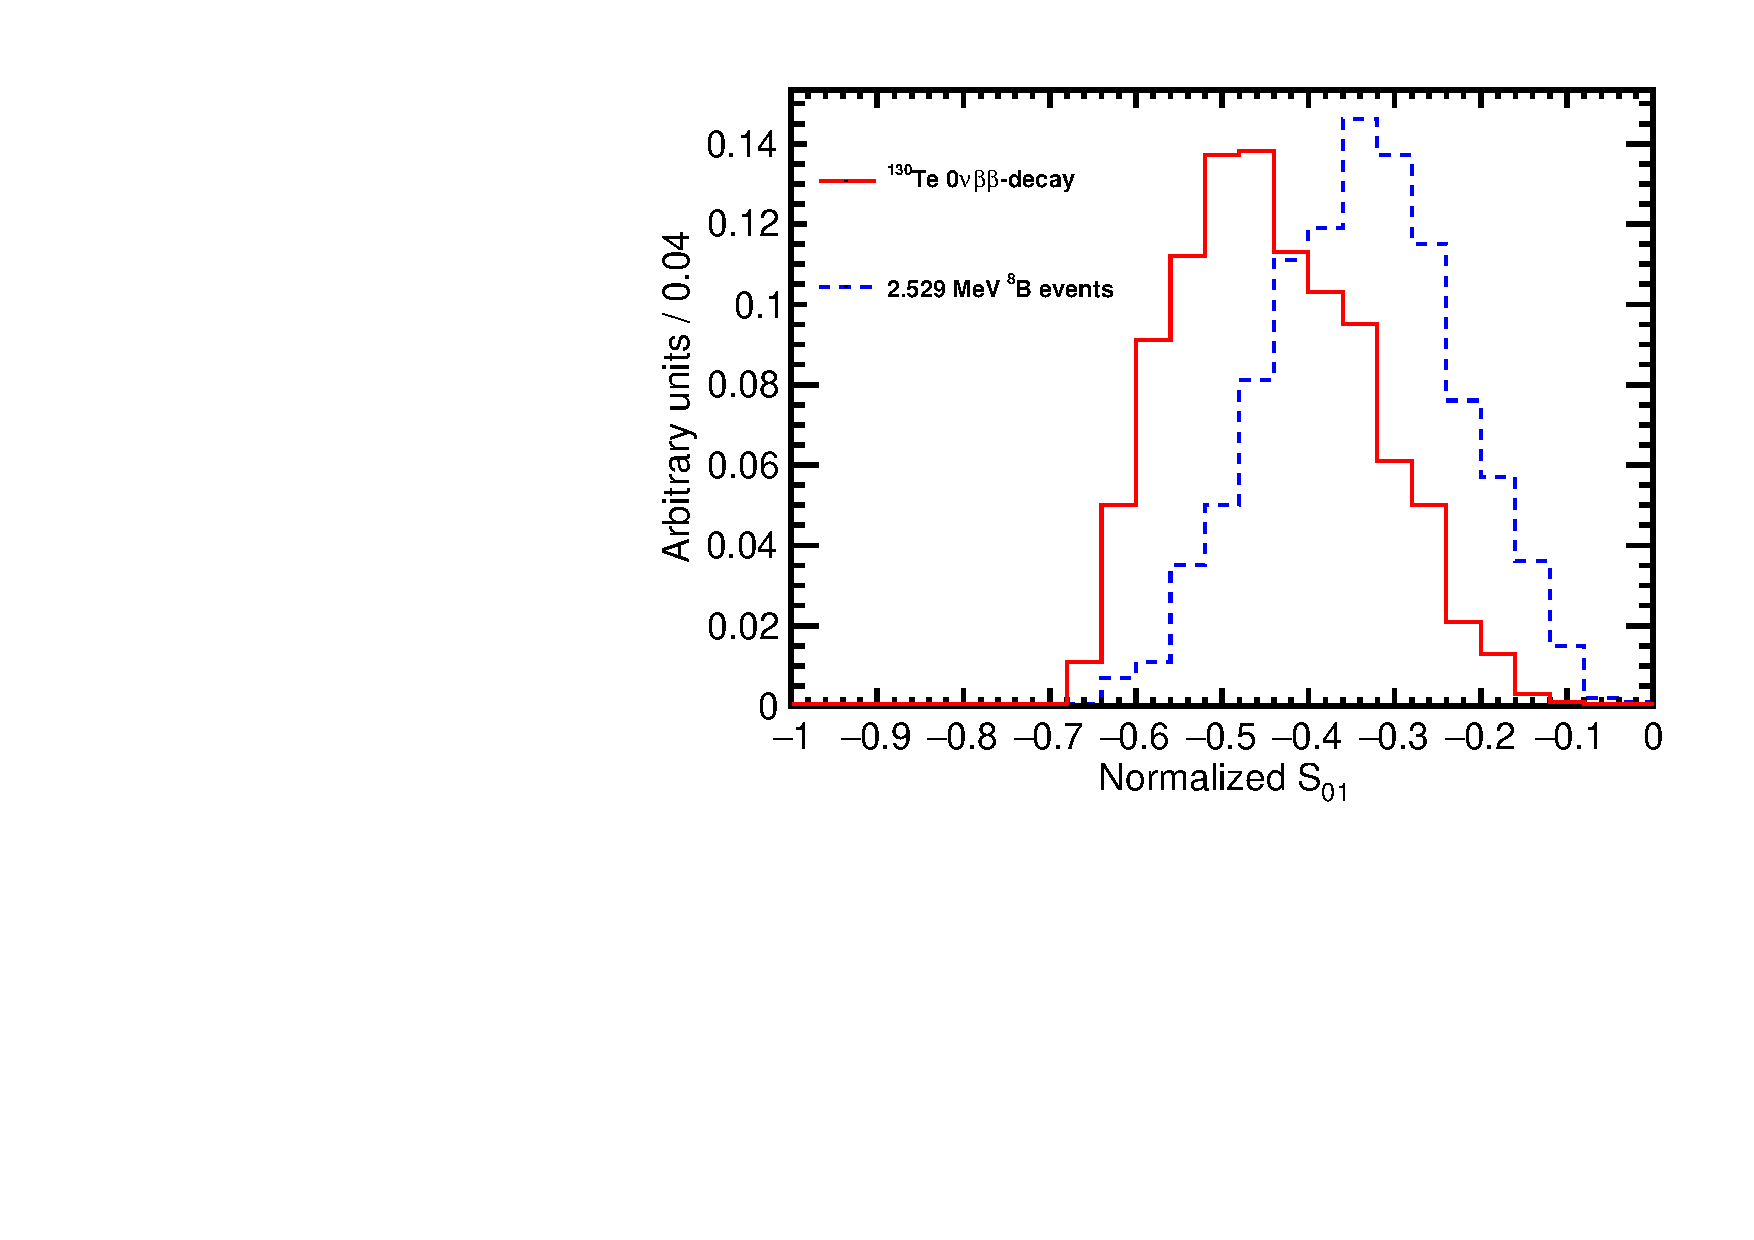
\includegraphics[width=0.49\textwidth]{hS01_allLight_VtxSmear3cm_VtxShiftX0cm_momDT1p0ns_rndVtx_3p0mSphere_SciRT5p0ns}
  \caption{The scintillation rise time constant is increased to
    $\tau_r=$5~ns compared to $\tau_r=$1~ns in the default detector
    model.  \emph{Left:} Scatter plot of $S_0$ versus $S_1$ for a
    simulation of 1000 signal (\emph{red crosses}) and background
    (\emph{blue triangles}) events. Event vertices are uniformly
    distributed within the fiducial volume, $R<3$~m.  Vertex is
    smeared with 3~cm resolution. Differential cut of $\Delta
    t=t^{phot}_{measured} - t^{phot}_{predicted}<$1~ns is applied to
    select early PE sample.  The default QE and 100\% photo-coverage
    is used in the simulation.  Black dashed line corresponds to a
    linear fit to define 1-D variable $S_{01}$ (see text for details).
    \emph{Right:} Comparison of the $S_{01}$ distribution between
    signal (\emph{red solid line}) and background (\emph{blue dashed
    line}).  $I_{overlap}$=0.64.}
\label{fig:SL_Te_SmearX3cm_momDT1ns_rndVtx_3p0m_SciRT5p0ns}
\end{figure*}

\clearpage

Figure~\ref{fig:Efficiency_Rejection} shows the
efficiency for 0\nbb~ signal and the rejection factor for \B~ neutrino
background for the default model (left-hand panel) 
and for the slower scintillator with
a 5-ns risetime (right-hand panel) as a function of the $S_{01}$
discriminant. We find a rejection factor of 2 for the default case at
70\% efficiency for signal. The rejection is increased to a factor of
3 for the 5-nsec risetime scintillator.

\begin{figure*}[h]
  \centering
  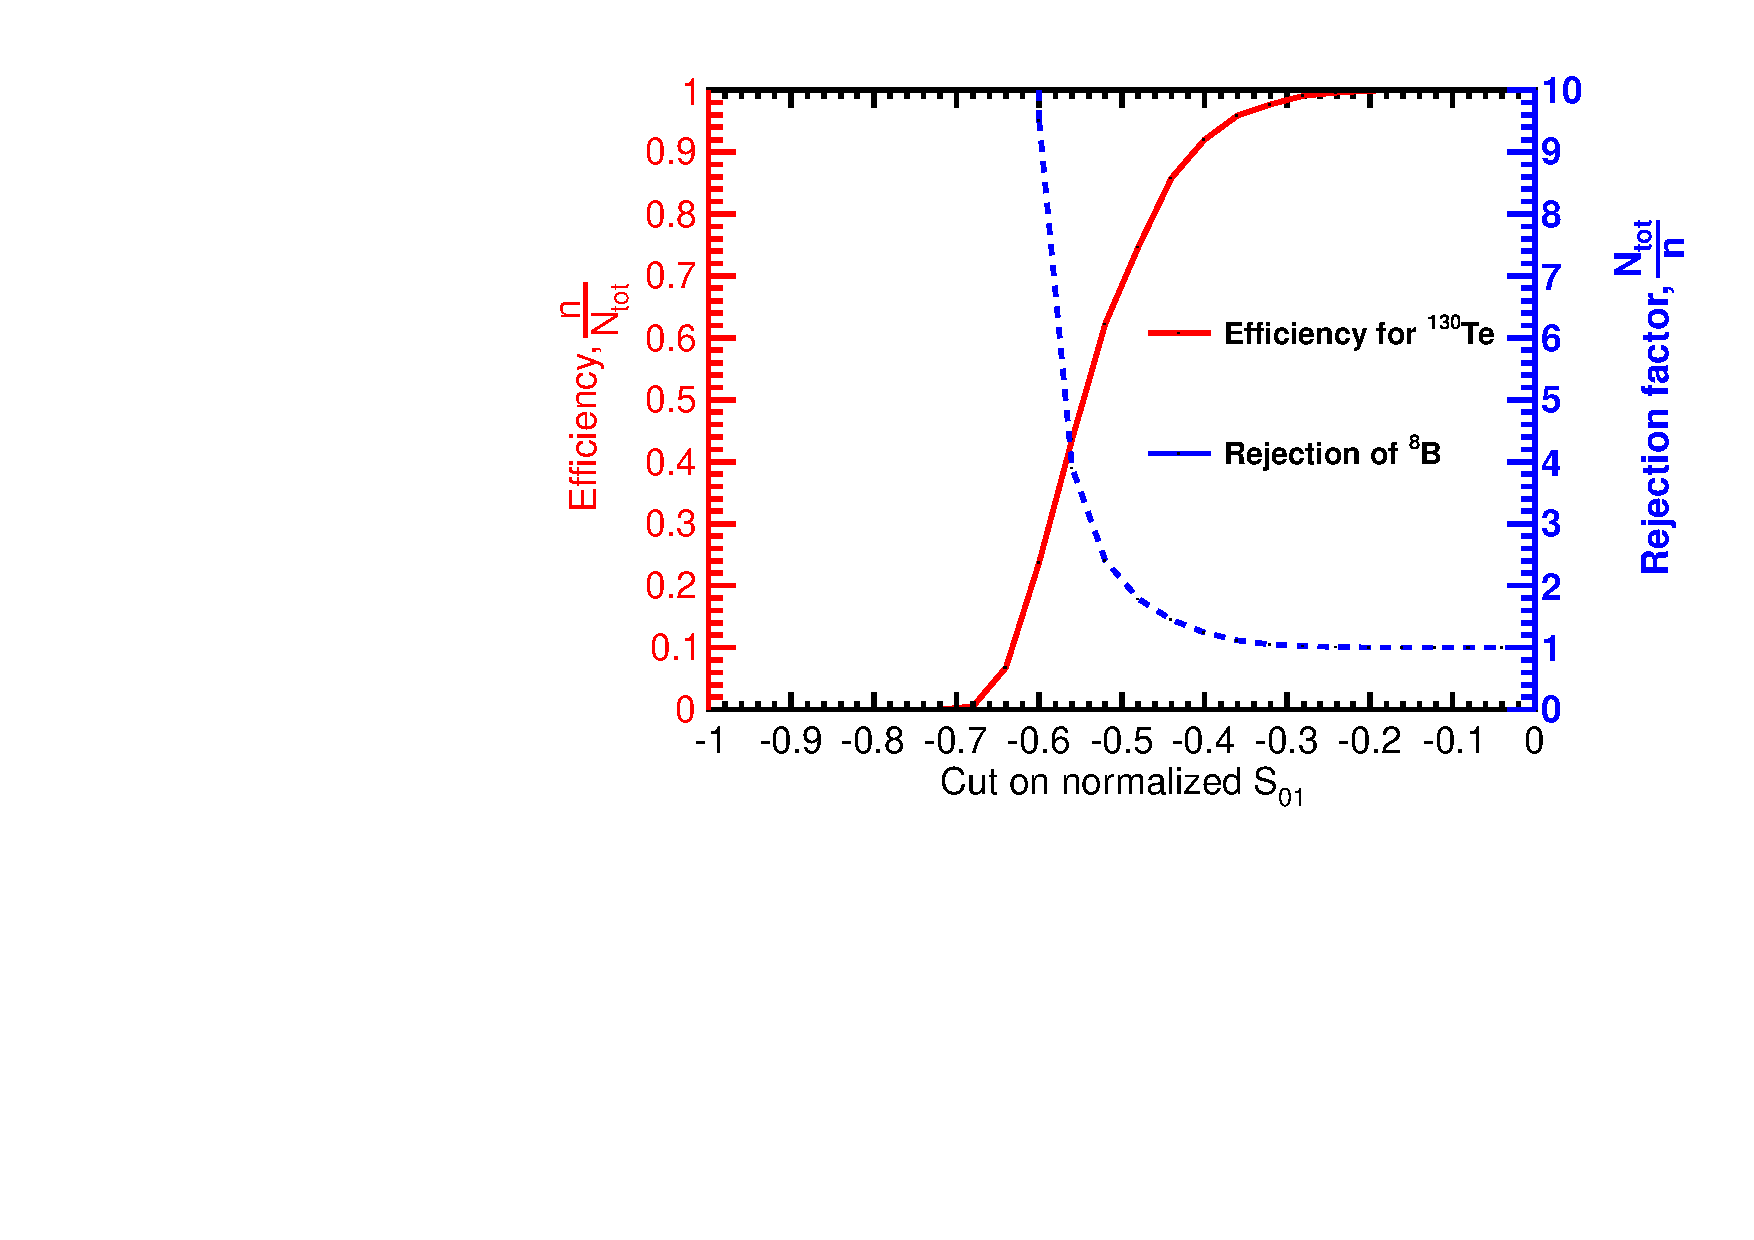
\includegraphics[width=0.49\textwidth]{hEff_real_case.pdf}
  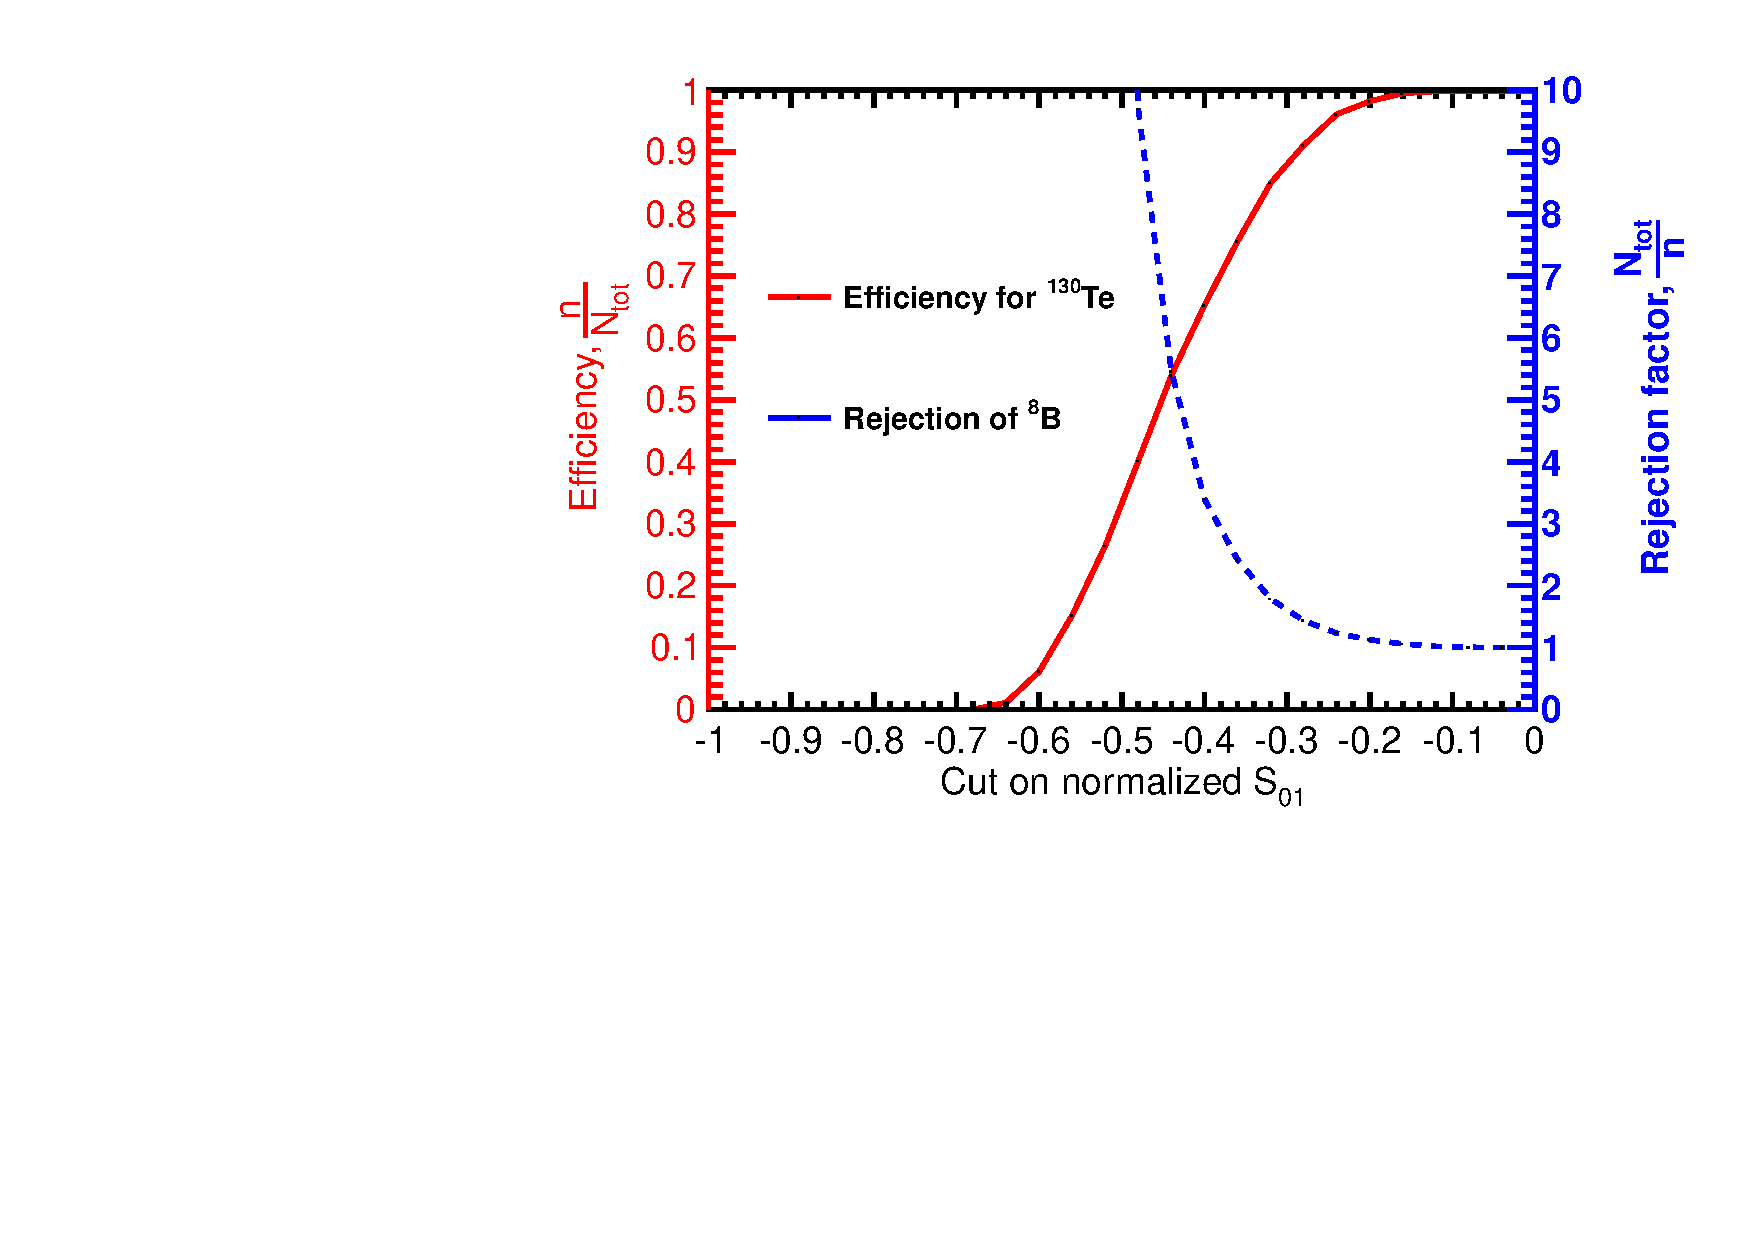
\includegraphics[width=0.49\textwidth]{hEff_5ns_case.pdf}
  \caption{ The efficiency for 0\nbb~ signal (left-hand scale )and the
rejection factor for \B neutrino background (right-hand scale) versus
$S_{01}$ for: \emph{Left:} the default model; and \emph{Right:} a
liquid scintillator with a 5-nsec risetime.}
\label{fig:Efficiency_Rejection}
\end{figure*}



%separation = 0.665755
%overlap = 0.642643


%Start:
%separation = 0.915454
%overlap = 0.521
%power = 1.76

%Middle:
%separation = 0.357271
%overlap = 0.793
%power = 0.45

%Final:
%separation = 0.665755
%overlap = 0.642643
%power = 1.04
